\documentclass[11pt,a4paper]{article}

\usepackage[utf8]{inputenc}
\usepackage{ngerman}
\usepackage{amsmath}
\usepackage{xcolor}
\definecolor{grey}{rgb}{0.9,0.9,0.9} % Colour of the box surrounding the title
% usenames allows you to use names of the default colors, the same 16 base colors as used in HTML. The dvipsnames allows you access to more colors, another 64, and svgnames allows access to about 150 colors. The initialization of "table" allows colors to be added to tables by placing the color command just before the table. If you need more colors, then you may also want to look at adding the x11names to the initialization section as well, this offers more than 300 colors, but you need to make sure your xcolor package is the most recent you can download.

\usepackage{scrextend} % addmargin
\usepackage{amssymb} % mathematische Symbole

\usepackage{tabularx} % erweiterte Tabellenoptionen
\newcolumntype{L}[1]{>{\raggedright\arraybackslash}p{#1}} % linksbündig mit Breitenangabe
\newcolumntype{C}[1]{>{\centering\arraybackslash}p{#1}} % zentriert mit Breitenangabe
\newcolumntype{R}[1]{>{\raggedleft\arraybackslash}p{#1}} % rechtsbündig mit Breitenangabe

\usepackage{endnotes}

\usepackage{graphicx}
\graphicspath{{Bilder/}}
\usepackage[autostyle=true,german=quotes]{csquotes}
\usepackage{enumitem}
\usepackage[T1]{fontenc}
\usepackage{textcomp}
\usepackage[sfdefault]{cabin}
\usepackage[onehalfspacing]{setspace}
%\renewcommand{\familydefault}{\sfdefault}

\date{\today}
\author{Marvin Janosch}
\title{Lastenheft}

\makeglossary

\begin{document}
	\renewcommand{\thefootnote}{\roman{footnote}}
	\let\footnote=\endnote %Synonym für footnote


	%\maketitle
	
	%----------------------------------------------------------------------------------------
	%	TITLE PAGE
	%----------------------------------------------------------------------------------------
	
	\begin{titlepage} % Suppresses displaying the page number on the title page and the subsequent page counts as page 1
		
		%------------------------------------------------
		%	Grey title box
		%------------------------------------------------
		
		\colorbox{grey}{
			\parbox[t]{0.93\textwidth}{ % Outer full width box
				\parbox[t]{0.91\textwidth}{ % Inner box for inner right text margin
					\raggedleft % Right align the text
					\fontsize{50pt}{50pt}\selectfont % Title font size, the first argument is the font size and the second is the line spacing, adjust depending on title length
					\vspace{0.7cm} % Space between the start of the title and the top of the grey box
					
					Pflichtenheft\\
					\fontsize{30pt}{50pt}\selectfont
					Autonomes Fahren\\
					\fontsize{30pt}{80pt}\selectfont
					Gruppe 3\\
					
					\vspace{0.7cm} % Space between the end of the title and the bottom of the grey box
				}
			}
		}
		
		\vfill % Space between the title box and author information
		
		%------------------------------------------------
		%	Author name and information
		%------------------------------------------------
		
		\parbox[t]{0.93\textwidth}{ % Box to inset this section slightly
			\raggedleft % Right align the text
			\large % Increase the font size
			{\Large Jan~Amann \\
			Khalid~Bellouch \\
			Marvin~Janosch \\
			Dennis~Szczepanski \\
			Jan~Philip~Wahle \\[8pt] % Extra space after name
			}
			Softwaretechnologie\\
			Bergische Universität Wuppertal \\[4pt] % Extra space before URL
			%\texttt{LaTeXTemplates.com}\\
			
			\hfill\rule{0.2\linewidth}{1pt}% Horizontal line, first argument width, second thickness
		}
		
	\end{titlepage}
	
	%----------------------------------------------------------------------------------------
	
	
	\pagebreak
	\begin{tabular}{|l|l|l|l|l|}
		\hline 
		\textbf{Version} & \textbf{Autor} & \textbf{Datum} & \textbf{Status} & \textbf{Kommentar} \\ 
		\hline 
		0.0 & Szczepanski & 22.10.17 & akzeptiert & Entwurf \\ 
		\hline 
		0.1 & Wahle & 22.10.17 & - & Format, Glossar, Kommentare \\ 
		\hline 
		0.2 & Amann & 31.10.17 & - & Vorschläge übernommen \\ 
		\hline 
		0.3 & Janosch & 02.11.17 & - & Latex, Anpassungen \\ 
		\hline 
	\end{tabular} 
	
	\pagebreak
	\tableofcontents
	
	%\begin{abstract}
	%	\begin{center}
	%		Zusammenfassung!
	%	\end{center}
	%\end{abstract}
	
	\renewcommand{\familydefault}{\sfdefault}

	
	\pagebreak
	\section{Zielbestimmung}
		Die fahrerlose Fortbewegung ist im Augenblick eines der relevantesten Themen der Automobilbranche. Bei dieser Art der Fortbewegung erkennt das Fahrzeug selbstständig, durch Einsatz von geeigneten Sensoren, zu welchem Augenblick sich ein Hindernis\footnote{\underline{\textbf{Hindernis, das}}: Ein Objekt variabler Größe, das sich innerhalb der zu simulierenden Strecke befindet. Dabei wird grundsätzlich zwischen sich bewegenden (dynamischen) und sich an einem bestimmten Punkt befindenden (statischen) Hindernissen unterschieden.} in welcher Position befindet und wählt autonom\footnote{\underline{\textbf{autonom}} (adj.): Ein System, dass ohne menschliche Eingriffe, also ganz autark agieren kann. In dem Fall das Fahrzeug.}, \underline{also ohne Einfluss eines menschlichen Führers des Fahrzeuges}, wie dieses umgangen werden soll.
		Der Auftraggeber möchte, dass ein solches autonomes Fahrzeug durch Software modelliert wird. Diese Software soll aus einem Editor\footnote{\underline{\textbf{Editor, der}}: Eine Benutzeroberfläche/Schnittstelle, durch die der ein Benutzer/Kunde die Möglichkeit bekommt, auch ohne jegliche Programmierkenntnisse, durch graphische Visualisierung, Teststrecken für eine Simulation zu erstellen. Dabei sind Streckenteile sowie Hindernisse vom Programmierer bereits vorgefertigt und können leicht zusammengeführt werden.} und einer Simulation\footnote{\underline{\textbf{Simulation, die}}: Ein Programmablauf, der es möglich macht eine bestimmte, vorgefertigte Situation, ablaufen zu lassen. In diesem Fall wird eine realitätsnahe Verkehrssituation simuliert, in der ein Fahrzeug autonom von einem Startpunkt zu einem Zielpunkt gelangen muss. } bestehen. Im Editor sollen Strecken und Hindernisse erstellt werden können. In der Simulation soll das Verhalten des Fahrzeuges auf eben dieser Strecke graphisch gezeigt werden können.

	\subsection{Musskriterien}
	\begin{itemize}
		\item Das Fahrzeug soll selbstständig die Teststrecke vom Start- zum Zielpunkt durchlaufen und dabei erfolgreich alle Hindernisse umgehen.
		\item Das Umgehen der Hindernisse soll nicht explizit Programmiert sein, sondern vom Fahrzeug durch eine Lernphase selbst erlernt werden.
		\item Das Fahrzeug soll eine Trägheit im physikalischen Sinne aufweisen. So gibt es beispielsweise eine Verzögerung zwischen Betätigung der Bremse und dem Stillstand des Fahrzeugs.
		\item Die Simulation soll sowohl zwei- als auch dreidimensional angezeigt werden können.
		\item In der Simulation soll es möglich sein verschiedene Strecken, so auch selbst erstellte, zu nutzen.
		\item Neben der Simulation soll das Projekt über einen Editor verfügen, in welchem Strecken erstellt, geladen, verändert und gespeichert werden können.
		\item Es soll möglich sein verschiedene Fahrzeuge mit unterschiedlichen Attributen zu erstellen.
	\end{itemize}
	
	\subsection{Wunschkriterien}
	\begin{itemize}
		\item Die Strecken sollen über Höheninformationen verfügen, welche das Fahrzeug beeinflussen. Bei positiver Steigung wird in diesem Fall das Fahrzeug nicht seine maximale Geschwindigkeit erreichen können. Bei negativer Steigung hingegen kann eine höhere Geschwindigkeit als auf der Ebene erreicht werden.
	\end{itemize}
	
	\subsection{Abgrenzungskriterien}
	\begin{itemize}
		\item Fahrzeuge, welche als Hindernis auf der Strecke sind, sollen sich nach einem Muster bewegen und dementsprechend nicht autonom fahren.
	\end{itemize}
	
	\pagebreak
	\section{Produkteinsatz}
	Das Produkt wird eingesetzt um den realen Straßenverkehr zu abstrahieren und realitätsnahe Szenarien zu simulieren. Das System soll dementsprechend mit großen Datenmengen trainiert werden, um später eine Lösung für die reale Welt zu bieten.
	
	\subsection{Anwendungsbereich}
	Simulation realer Ereignisse im Straßenverkehr
	\subsection{Zielgruppe}
	Ingenieure, Fachpersonal
	\subsection{Betriebsbedingung}
	Büroumgebung
	
	\pagebreak
	\section{Produktübersicht}
	\begin{figure}[ht]
		\centering
		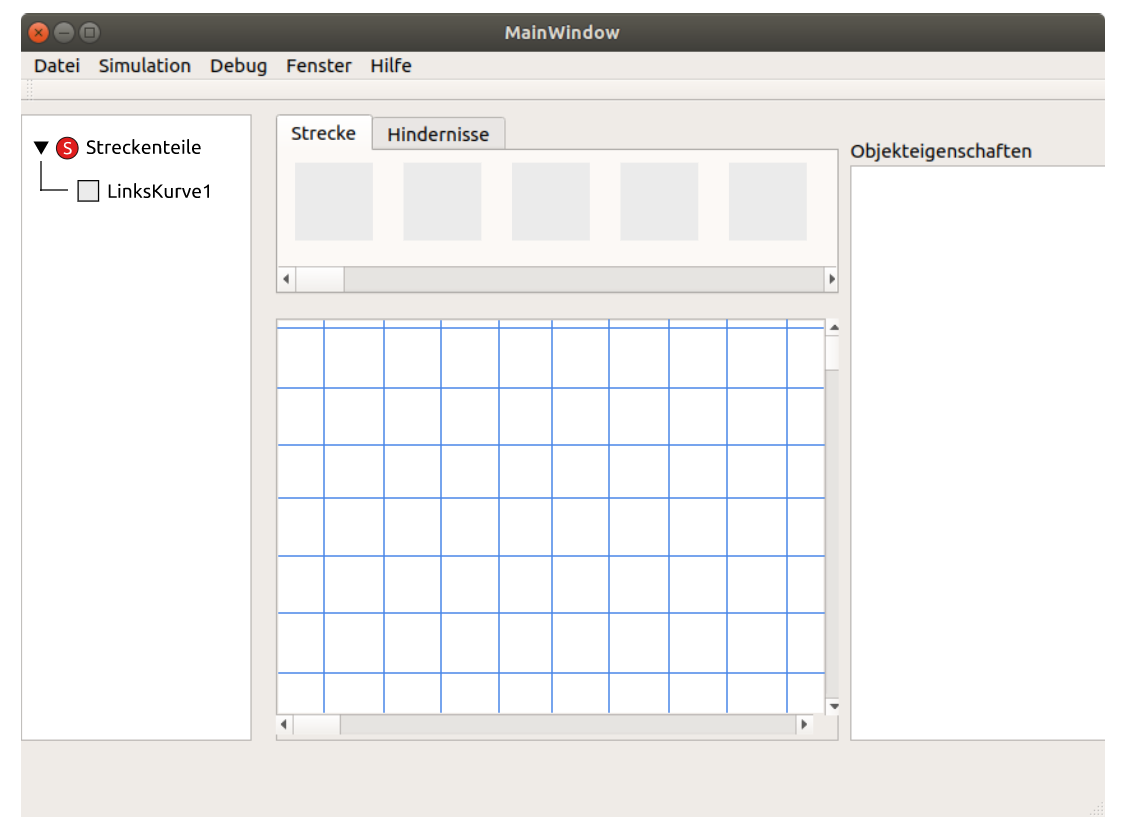
\includegraphics[width=\textwidth]{prototyp1}
		\caption[Netztopologie elektrische Versorgung]{Prototyp des Editors.}
		\label{fig:prot1}
	\end{figure}

	
	\pagebreak
	\section{Produktfunktionen}
	\subsection{Editor}
	\noindent\large\textbf{/F10/} (/LF10/)
	\normalsize\\
	\begin{addmargin}{0.1 \textwidth}
		\textbf{Prozess:} Erstellung sowie Änderung von Strecken.\\
		\textbf{Ziel:} Es wird eine Strecke mit den vordefinierten Streckenabschnitten erstellt.\\
		\textbf{Kategorie:} primär\\
		\textbf{Vorbedingung:} -\\
		\textbf{Nachbedingung Erfolg:} Die Strecke kann gespeichert werden.\\
		\textbf{Nachbedingung Fehlschlag:} Mitteilung an den Benutzer mit der Beschreibung des Fehlers.\\
		\textbf{Akteure:} Kunde, Firma\\
		\\
		\begin{minipage}{\textwidth}
			\textbf{Beschreibung:}
			\begin{enumerate}
				\item Größe der Strecke wird definiert.
				\item Strecke wird mithilfe der gegebenen Streckenabschnitte erstellt.
				\item Start- und Zielpunkt werden gesetzt.\\
			\end{enumerate}
		\end{minipage}
		\\
		\begin{minipage}{\textwidth}
			\textbf{Erweiterung:}
			\begin{enumerate}
				\item Größe der Strecke wird geändert.
				\item Anordnung der Streckenabschnitte wird geändert.
				\item Start- und Zielpunkt werden verschoben.\\
			\end{enumerate}
		\end{minipage}
	\end{addmargin}

	\noindent\large\textbf{/F20/} (/LF20/)
	\normalsize\\
	\begin{addmargin}{0.1 \textwidth}
		\textbf{Prozess:} Speichern einer Strecke.\\
		\textbf{Ziel:} Eine erstellte Strecke wird in einer Datei gespeichert, welche daraufhin von der Simulation genutzt werden kann, aber auch wieder in den Streckeneditor geladen werden kann.\\
		\textbf{Kategorie:} Primär\\
		\textbf{Vorbedingung:} Strecke muss zuvor erstellt worden sein.\\
		\textbf{Nachbedingung Erfolg:} Strecke kann von Simulation/Editor geladen werden.\\
		\textbf{Nachbedingung Fehlschlag:} Mitteilung an den Benutzer mit der Beschreibung des Fehlers.\\
		\textbf{Akteure:} Kunde, Firma\\
		\\
		\begin{minipage}{\textwidth}
			\textbf{Beschreibung:}
			\begin{enumerate}
				\item Es wird eine Datei angelegt, welche alle relevanten Details zur Strecke beinhaltet.\\
			\end{enumerate}
		\end{minipage}
	\end{addmargin}
	
	\noindent\large\textbf{/F30/} (/LF30/)
	\normalsize\\
	\begin{addmargin}{0.1 \textwidth}
		\textbf{Prozess:} Erstellen und Ändern eines Fahrzeuges.\\
		\textbf{Ziel:} Es wird ein Fahrzeug erstellt, welches in der Simulation genutzt werden kann.\\
		\textbf{Kategorie:} Primär\\
		\textbf{Vorbedingung:} -\\
		\textbf{Nachbedingung Erfolg:}  Fahrzeug kann von Simulation genutzt werden.\\
		\textbf{Nachbedingung Fehlschlag:} Mitteilung an den Benutzer mit der Beschreibung des Fehlers.\\
		\textbf{Akteure:} Kunde, Firma\\
		\\
		\begin{minipage}{\textwidth}
			\textbf{Beschreibung:}
			\begin{enumerate}
				\item Es werden alle relevanten Daten zum Fahrzeug abgefragt (Größe, Maximale Geschwindigkeit, Bremsverhalten).
				\item Fahrzeug wird in einer Datei für spätere Benutzung gespeichert.\\
			\end{enumerate}
		\end{minipage}
		\\
		\begin{minipage}{\textwidth}
			\textbf{Erweiterung:}
			\begin{enumerate}
				\item Es werden Attribute\footnote{\underline{\textbf{Attribut, das}}: Eine Eigenschaft, die einen Sachverhalt oder in dem Falle ein Objekt eindeutig beschreiben. Für ein Fahrzeug wären klassische Attribute: Höchstgeschwindigkeit, Leistung, Abmessungen, etc.} des Fahrzeuges geändert.\\
			\end{enumerate}
		\end{minipage}
	\end{addmargin}
	
	\noindent\large\textbf{/F40/} (/LF40/)
	\normalsize\\
	\begin{addmargin}{0.1 \textwidth}
		\textbf{Prozess:} Erstellung und Löschung von statischen und dynamischen Objekten.\\
		\textbf{Ziel:} Es werden vordefinierte Hindernisse zu der Strecke hinzugefügt oder gelöscht.\\
		\textbf{Kategorie:} Primär\\
		\textbf{Vorbedingung:} Strecke muss zuvor erstellt worden sein.\\
		\textbf{Nachbedingung Erfolg:} Strecke kann gespeichert werden.\\
		\textbf{Nachbedingung Fehlschlag:} Mitteilung an den Benutzer mit der Beschreibung des Fehlers.\\
		\textbf{Akteure:} Kunde, Firma\\
		\\
		\begin{minipage}{\textwidth}
			\textbf{Beschreibung:}
			\begin{enumerate}
				\item Elemente werden der Strecke hinzugefügt.
				\item Es wird getestet, ob die Strecke noch passierbar ist.\\
			\end{enumerate}
		\end{minipage}
		\begin{minipage}{\textwidth}
			\textbf{Erweiterung:}
			\begin{enumerate}
				\item Elemente werden von der Strecke entfernt.\\
			\end{enumerate}
		\end{minipage}
	\end{addmargin}
	
	\subsection{Simulation}
	\noindent\large\textbf{/F50/} (/LF20/)
	\normalsize\\
	\begin{addmargin}{0.1 \textwidth}
		\textbf{Prozess:} Laden einer Strecke in die Simulation.\\
		\textbf{Ziel:} Eine zuvor erstellte Strecke wird von der Simulation geladen, damit diese durchlaufen werden kann.\\
		\textbf{Kategorie:} Primär\\
		\textbf{Vorbedingung:} Strecke muss zuvor gespeichert worden sein.\\
		\textbf{Nachbedingung Erfolg:} Simulation kann gestartet werden.\\
		\textbf{Nachbedingung Fehlschlag:} Mitteilung an den Benutzer mit der Beschreibung des Fehlers.\\
		\\
		\begin{minipage}{\textwidth}
			\textbf{Beschreibung:}
			\begin{enumerate}
				\item Streckendatei wird ausgewählt.
				\item Simulation lädt diese Datei und stellt sie grafisch dar.\\
			\end{enumerate}
		\end{minipage}
	\end{addmargin}

	\noindent\large\textbf{/F60/} (/LF50/)
	\normalsize\\
	\begin{addmargin}{0.1 \textwidth}
		\textbf{Prozess:} Starten, pausieren und beenden der Simulation.\\
		\textbf{Ziel:} Die Simulation wird gestartet und das Fahrzeug versucht die gegebene Strecke zu durchfahren.\\
		\textbf{Vorbedingung:} Strecke muss zuvor geladen worden sein.\\
		\textbf{Nachbedingung Erfolg:} Simulation war erfolgreich. Das Fahrzeug ist mit dem aktuellen Lernstand in der Lage die Strecke zu durchfahren.\\
		\textbf{Nachbedingung Fehlschlag:} Fahrzeug ist mit aktuellen Lernstand nicht in der Lage die Strecke zu durchfahren. Weitere Lernphasen nötig.\\
		\\
		\begin{minipage}{\textwidth}
			\textbf{Beschreibung:}
			\begin{enumerate}
				\item Simulation wird gestartet.
				\item Simulation läuft so lange, bis Fahrzeug den Zielpunkt erreicht hat oder eine Kollision\footnote{\underline{\textbf{Kollision, die}}: Im klassischen Sinne ein Zusammenstoß zweier Objekte. In diesem Fall einer, der Objekte Fahrzeug und Fahrbahn bzw. Fahrzeug und Hindernis. Diese Kollision wird durch eine Berührung der beiden beschreibenden mathematischen Funktionen gekennzeichnet.} besteht.\\
			\end{enumerate}
		\end{minipage}
		\begin{minipage}{\textwidth}
			\textbf{Alternative:}
			\begin{enumerate}
				\item Simulation wird pausiert.
				\item Simulation wird vom Benutzer gestoppt.\\
			\end{enumerate}
		\end{minipage}
	\end{addmargin}

	\noindent\large\textbf{/F70/} (/LF60/)
	\normalsize\\
	\begin{addmargin}{0.1 \textwidth}
		\textbf{Prozess:} Fahrzeug und Objekte verhalten sich auf der Strecke gemäß ihren Attributen.\\
		\textbf{Ziel:} Bei gestarteter Simulation bewegt sich das Fahrzeug und andere Objekte, so wie es ihre Attribute festlegen.\\
		\textbf{Vorbedingung:} Simulation muss gestartet worden sein.\\
		\textbf{Nachbedingung Erfolg:} Bewegung von Fahrzeug und Objekten werden durch ihre Trägheit und ihr Verhalten beeinflusst.\\
		\textbf{Nachbedingung Fehlschlag:} Objekte Bewegen sich nicht wie spezifiziert.\\
		\\
		\begin{minipage}{\textwidth}
			\textbf{Beschreibung:}
			\begin{enumerate}
				\item Simulation wird gestartet.
				\item Fahrzeug reagiert auf Bremssituationen gemäß seiner Attribute.\\
			\end{enumerate}
		\end{minipage}
		\begin{minipage}{\textwidth}
			\textbf{Erweiterung:}
			\begin{enumerate}
				\item Andere Fahrzeuge bewegen sich ihrem definierten Verhalten entsprechend.\\
			\end{enumerate}
		\end{minipage}
	\end{addmargin}

	\noindent\large\textbf{/F80/} (/LF70/)
	\normalsize\\
	\begin{addmargin}{0.1 \textwidth}
		\textbf{Prozess:} Fahrzeuge lernen anhand durchlaufener Strecken, wie sie sich auf nicht durchlaufenen Strecken verhalten sollen.\\
		\textbf{Vorbedingung:} -\\
		\textbf{Nachbedingung Erfolg:} Fahrzeug durchläuft neue Strecken eigenständig und bereits bekannte Strecken mit einer höheren Fitness\footnote{\underline{\textbf{Fitness}} (engl.): Eine Maßeinheit, die beschreibt, welchen Erfolg die Simulation bzw. das Fahrzeug in der Simulation hatte. Dies kann beschrieben werden durch die Strecke, die das Fahrzeug ohne Kollision zurückgelegt hat.}.\\
		\textbf{Nachbedingung Fehlschlag:} Das Fahrzeug besitzt kein Lernverhalten.\\
		\\
		\begin{minipage}{\textwidth}
			\textbf{Beschreibung:}
			\begin{enumerate}
				\item Simulation wird durchlaufen.
				\item Relevante Daten der Simulation werden gespeichert und ausgewertet.\\
			\end{enumerate}
		\end{minipage}
	\end{addmargin}
	
	\pagebreak
	\section{Produktdaten}
	\noindent\large\textbf{/D10/} (/LD10/) Streckendaten
	\normalsize \\
	\begin{addmargin}{0.1 \textwidth}
		Dimension ($N \times M, \text{mit } N, M \in \mathbb{N}$) der Karte, Anzahl der Felder, Feldart, Objekte, Steigungen.\\
	\end{addmargin}

	\noindent\large\textbf{/D20/} (/LD20/) Fahrzeug
	\normalsize \\
	\begin{addmargin}{0.1 \textwidth}
		Statisch\footnote{\underline{\textbf{statische Fahrzeugdaten}}: unveränderliche Eigenschaften des Fahrzeugs wie Größe oder Geschwindigkeit.}: Maximale Geschwindigkeit, Beschleunigungsverhalten, Bremsverhalten, Größe. \\
		Dynamisch\footnote{\underline{\textbf{dynamische Fahrzeugdaten}}: Fahrzeugdaten, wie Sensoren oder Fitness, die veränderlich sind.}: Sensoren, Fitness, Abstand zu Begrenzungen Abstand zu Objekten.\\
	\end{addmargin}

	\noindent\large\textbf{/D30/} (/LD30/) Fitness
	\normalsize \\
	\begin{addmargin}{0.1 \textwidth}
		Zurückgelegte Strecke ohne Kollision, statische Fahrzeugdaten, dynamische Fahrzeugdaten.\\
	\end{addmargin}

	\noindent\large\textbf{/D40/} (/LD40/) Lerndaten
	\normalsize \\
	\begin{addmargin}{0.1 \textwidth}
		Tensorflow.\\
	\end{addmargin}

	\pagebreak
	\section{Produktleistungen}
	\noindent\large\textbf{/L10/} (/LL10/) 
	\normalsize \\
	\begin{addmargin}{0.1 \textwidth}
		Die Reaktionszeit des Fahrzeugs hat höchste Priorität und soll in Echtzeit realisiert werden.\\
	\end{addmargin}

	\noindent\large\textbf{/L20/} (/LL20/) 
	\normalsize \\
	\begin{addmargin}{0.1 \textwidth}
		Der letztendliche Lernprozess sollte sich auf 24 Stunden und weniger als 10 Strecken beschränken.\\
	\end{addmargin}
	
	\noindent\large\textbf{/L30/} (/LL30/) 
	\normalsize \\
	\begin{addmargin}{0.1 \textwidth}
		Das Laden sowie Speichern von Strecken sollte unter 5 Sekunden liegen.\\
	\end{addmargin}

	\section{Qualitätsanforderungen}
	\begin{center}
		\begin{tabular}{|l|C{50pt}|C{50pt}|C{50pt}|}
			\hline 
			\textbf{Qualität} & \textbf{Sehr gut} & \textbf{Gut} & \textbf{Normal} \\ 
			\hline 
			Funktionalität & X &  &  \\ 
			\hline 
			Zuverlässigkeit &  & X &  \\ 
			\hline 
			Benutzbarkeit &  &  & X \\ 
			\hline 
			Effizienz &  &  & X \\ 
			\hline 
			Änderbarkeit &  &  & X \\ 
			\hline 
			Übertragbarkeit &  & X &  \\ 
			\hline 
		\end{tabular} 
	\end{center}

	\section{Benutzeroberfläche}
	\noindent\large\textbf{/B10/} Editor
	\normalsize \\
	\noindent\large\textbf{/B20/} Simulation 2D
	\normalsize \\
	\noindent\large\textbf{/B30/} Simulation 3D
	\normalsize \\

	\section{Nicht-funktionale Anforderungen}
	\noindent\large\textbf{/NA10/}
	\normalsize \\
	\begin{addmargin}{0.1 \textwidth}
		Das Produkt soll für Entwickler leicht erweiterbar sein. Es soll ohne große Schwierigkeiten möglich sein, neue Feldtypen oder Objekttypen zu erstellen.\\
	\end{addmargin}

	\section{Technische Produktumgebung}
	\subsection{Software}
		\begin{enumerate}
			\item Qt Creator
			\item LaTeX
			\item Slack
			\item GitHub
		\end{enumerate}
	\subsection{Hardware}
		\begin{itemize}
			\item Windows, macOS, Linux
			\item 2 GHz CPU
			\item 4 GB RAM
			\item Nvidia CUDA-fähige GPU
		\end{itemize}
	
	\pagebreak	
	\renewcommand{\notesname}{\section{Glossar}}
	\begingroup
	\parindent 0pt
	\parskip 2ex
	\def\enotesize{\normalsize}
	\theendnotes
	\endgroup
	
\end{document}